% Options for packages loaded elsewhere
% Options for packages loaded elsewhere
\PassOptionsToPackage{unicode}{hyperref}
\PassOptionsToPackage{hyphens}{url}
%
\documentclass[
  ignorenonframetext,
  aspectratio=169,
]{beamer}
\newif\ifbibliography
\usepackage{pgfpages}
\setbeamertemplate{caption}[numbered]
\setbeamertemplate{caption label separator}{: }
\setbeamercolor{caption name}{fg=normal text.fg}
\beamertemplatenavigationsymbolsempty
% remove section numbering
\setbeamertemplate{part page}{
  \centering
  \begin{beamercolorbox}[sep=16pt,center]{part title}
    \usebeamerfont{part title}\insertpart\par
  \end{beamercolorbox}
}
\setbeamertemplate{section page}{
  \centering
  \begin{beamercolorbox}[sep=12pt,center]{section title}
    \usebeamerfont{section title}\insertsection\par
  \end{beamercolorbox}
}
\setbeamertemplate{subsection page}{
  \centering
  \begin{beamercolorbox}[sep=8pt,center]{subsection title}
    \usebeamerfont{subsection title}\insertsubsection\par
  \end{beamercolorbox}
}
% Prevent slide breaks in the middle of a paragraph
\widowpenalties 1 10000
\raggedbottom
\usepackage{iftex}
\ifPDFTeX
  \usepackage[T1]{fontenc}
  \usepackage[utf8]{inputenc}
  \usepackage{textcomp} % provide euro and other symbols
\else % if luatex or xetex
  \usepackage{unicode-math} % this also loads fontspec
  \defaultfontfeatures{Scale=MatchLowercase}
  \defaultfontfeatures[\rmfamily]{Ligatures=TeX,Scale=1}
\fi
\usepackage{lmodern}

\usetheme[]{metropolis}
\ifPDFTeX\else
  % xetex/luatex font selection
\fi
% Use upquote if available, for straight quotes in verbatim environments
\IfFileExists{upquote.sty}{\usepackage{upquote}}{}
\IfFileExists{microtype.sty}{% use microtype if available
  \usepackage[]{microtype}
  \UseMicrotypeSet[protrusion]{basicmath} % disable protrusion for tt fonts
}{}
\makeatletter
\@ifundefined{KOMAClassName}{% if non-KOMA class
  \IfFileExists{parskip.sty}{%
    \usepackage{parskip}
  }{% else
    \setlength{\parindent}{0pt}
    \setlength{\parskip}{6pt plus 2pt minus 1pt}}
}{% if KOMA class
  \KOMAoptions{parskip=half}}
\makeatother


\usepackage{longtable,booktabs,array}
\usepackage{calc} % for calculating minipage widths
\usepackage{caption}
% Make caption package work with longtable
\makeatletter
\def\fnum@table{\tablename~\thetable}
\makeatother
\usepackage{graphicx}
\makeatletter
\newsavebox\pandoc@box
\newcommand*\pandocbounded[1]{% scales image to fit in text height/width
  \sbox\pandoc@box{#1}%
  \Gscale@div\@tempa{\textheight}{\dimexpr\ht\pandoc@box+\dp\pandoc@box\relax}%
  \Gscale@div\@tempb{\linewidth}{\wd\pandoc@box}%
  \ifdim\@tempb\p@<\@tempa\p@\let\@tempa\@tempb\fi% select the smaller of both
  \ifdim\@tempa\p@<\p@\scalebox{\@tempa}{\usebox\pandoc@box}%
  \else\usebox{\pandoc@box}%
  \fi%
}
% Set default figure placement to htbp
\def\fps@figure{htbp}
\makeatother





\setlength{\emergencystretch}{3em} % prevent overfull lines

\providecommand{\tightlist}{%
  \setlength{\itemsep}{0pt}\setlength{\parskip}{0pt}}



 


% ============================================================
%  Econ 2203 — Beamer Metropolis Theme Preamble
%  Course: International Trade and Policy in Agriculture
%  Instructor: Nithin M, Department of Development Economics
% ============================================================

% MUST be first: load Metropolis theme before \metroset and colour overrides
\usetheme{metropolis}

% Only load packages not already provided by pandoc's beamer template
\usepackage{amsmath,amssymb}

% ---- Brand colours -----------------------------------------
\definecolor{brandblue}{HTML}{012169}
\definecolor{brandgold}{HTML}{B9975B}
\definecolor{lightblue}{HTML}{E8EDF5}

% ---- Metropolis colour overrides ---------------------------
% Main palette
\setbeamercolor{normal text}{fg=black,bg=white}
\setbeamercolor{alerted text}{fg=brandgold}
\setbeamercolor{example text}{fg=brandblue!70!black}

% Title slide
\setbeamercolor{title}{fg=white,bg=brandblue}
\setbeamercolor{subtitle}{fg=brandgold}
\setbeamercolor{author}{fg=white}
\setbeamercolor{institute}{fg=brandgold!80!white}
\setbeamercolor{date}{fg=white}
\setbeamercolor{title page header}{fg=white,bg=brandblue}

% Frametitle bar
\setbeamercolor{frametitle}{fg=white,bg=brandblue}

% Progress bar → gold
\setbeamercolor{progress bar}{fg=brandgold,bg=brandblue!30}
\setbeamercolor{title separator}{fg=brandgold}
\setbeamercolor{progress bar in head/foot}{fg=brandgold,bg=brandblue!20}
\setbeamercolor{progress bar in section page}{fg=brandgold,bg=brandblue!20}

% Blocks
\setbeamercolor{block title}{bg=brandblue,fg=white}
\setbeamercolor{block body}{bg=lightblue,fg=black}
\setbeamercolor{block title alerted}{bg=brandgold,fg=white}
\setbeamercolor{block body alerted}{bg=brandgold!12,fg=black}
\setbeamercolor{block title example}{bg=brandblue!70!black,fg=white}
\setbeamercolor{block body example}{bg=brandblue!8,fg=black}

% Structure / lists
\setbeamercolor{structure}{fg=brandblue}
\setbeamercolor{section in toc}{fg=brandblue}
\setbeamercolor{itemize item}{fg=brandblue}
\setbeamercolor{itemize subitem}{fg=brandgold}
\setbeamercolor{enumerate item}{fg=brandblue}
\setbeamercolor{description item}{fg=brandblue}

% ---- Metropolis options ------------------------------------
\metroset{
  progressbar    = frametitle,   % gold bar under frametitle
  sectionpage    = none,
  numbering      = fraction,
  block          = fill
}

% ---- Fonts (Metropolis uses Fira Sans; fallback gracefully) -
\setbeamerfont{title}{size=\Large,series=\bfseries}
\setbeamerfont{subtitle}{size=\normalsize,series=\mdseries}
\setbeamerfont{frametitle}{size=\large,series=\bfseries}
\setbeamerfont{block title}{size=\normalsize,series=\bfseries}
\setbeamerfont{caption}{size=\footnotesize}

% ---- Footer: course info + slide number --------------------
\setbeamertemplate{footline}{%
  \begin{beamercolorbox}[wd=\paperwidth,ht=2.0ex,dp=1ex]{footline}%
    \hspace{0.8em}%
    {\footnotesize\color{brandblue!60}%
      Econ 2203 \textbar{} International Trade and Policy in Agriculture
      \hfill Nithin M \hfill
      \insertframenumber{}/\inserttotalframenumber\hspace{0.8em}}%
  \end{beamercolorbox}%
}

% ---- Misc --------------------------------------------------
\setlength{\parskip}{0.25em}
\setbeamertemplate{navigation symbols}{}

% tighter column sep for side-by-side content
\setlength{\columnsep}{0.8em}

% Fix: make \label truly robust in moving arguments (Quarto generates
% \caption{\label{fig-xxx}...} which crashes Metropolis in batchmode).
% DeclareRobustCommand creates a self-protecting robust version.
\makeatletter
\let\quarto@originallabel\label
\DeclareRobustCommand*{\label}[1]{\quarto@originallabel{#1}}
\makeatother

% Prevent figures from overflowing Beamer frames.
% width=\linewidth: scale to text width (already Quarto default);
% height=0.6\textheight: cap height so figures never push past the frame bottom.
% keepaspectratio: never distort — whichever constraint binds first wins.
\setkeys{Gin}{width=\linewidth,height=0.6\textheight,keepaspectratio}
\makeatletter
\@ifpackageloaded{tcolorbox}{}{\usepackage[skins,breakable]{tcolorbox}}
\@ifpackageloaded{fontawesome5}{}{\usepackage{fontawesome5}}
\definecolor{quarto-callout-color}{HTML}{909090}
\definecolor{quarto-callout-note-color}{HTML}{0758E5}
\definecolor{quarto-callout-important-color}{HTML}{CC1914}
\definecolor{quarto-callout-warning-color}{HTML}{EB9113}
\definecolor{quarto-callout-tip-color}{HTML}{00A047}
\definecolor{quarto-callout-caution-color}{HTML}{FC5300}
\definecolor{quarto-callout-color-frame}{HTML}{acacac}
\definecolor{quarto-callout-note-color-frame}{HTML}{4582ec}
\definecolor{quarto-callout-important-color-frame}{HTML}{d9534f}
\definecolor{quarto-callout-warning-color-frame}{HTML}{f0ad4e}
\definecolor{quarto-callout-tip-color-frame}{HTML}{02b875}
\definecolor{quarto-callout-caution-color-frame}{HTML}{fd7e14}
\makeatother
\makeatletter
\@ifpackageloaded{caption}{}{\usepackage{caption}}
\AtBeginDocument{%
\ifdefined\contentsname
  \renewcommand*\contentsname{Table of contents}
\else
  \newcommand\contentsname{Table of contents}
\fi
\ifdefined\listfigurename
  \renewcommand*\listfigurename{List of Figures}
\else
  \newcommand\listfigurename{List of Figures}
\fi
\ifdefined\listtablename
  \renewcommand*\listtablename{List of Tables}
\else
  \newcommand\listtablename{List of Tables}
\fi
\ifdefined\figurename
  \renewcommand*\figurename{Figure}
\else
  \newcommand\figurename{Figure}
\fi
\ifdefined\tablename
  \renewcommand*\tablename{Table}
\else
  \newcommand\tablename{Table}
\fi
}
\@ifpackageloaded{float}{}{\usepackage{float}}
\floatstyle{ruled}
\@ifundefined{c@chapter}{\newfloat{codelisting}{h}{lop}}{\newfloat{codelisting}{h}{lop}[chapter]}
\floatname{codelisting}{Listing}
\newcommand*\listoflistings{\listof{codelisting}{List of Listings}}
\makeatother
\makeatletter
\makeatother
\makeatletter
\@ifpackageloaded{caption}{}{\usepackage{caption}}
\@ifpackageloaded{subcaption}{}{\usepackage{subcaption}}
\makeatother

\usepackage{bookmark}
\IfFileExists{xurl.sty}{\usepackage{xurl}}{} % add URL line breaks if available
\urlstyle{same}
\hypersetup{
  pdftitle={Theories of Trade II: Comparative Advantage},
  pdfauthor={Nithin M},
  hidelinks,
  pdfcreator={LaTeX via pandoc}}


\title{Theories of Trade II: Comparative Advantage}
\subtitle{Econ 2203 \textbar{} International Trade and Policy in
Agriculture}
\author{Nithin M}
\date{2026-05-16}
\institute{Department of Development Economics}

\begin{document}
\frame{\titlepage}


\section{Part I: The Problem with Absolute
Advantage}\label{part-i-the-problem-with-absolute-advantage}

\begin{frame}{Recap: The Gap in Smith's Theory}
\phantomsection\label{recap-the-gap-in-smiths-theory}
\textbf{Last lecture:} Adam Smith argued that countries should export
goods they produce \emph{absolutely} more efficiently.

\textbf{But this raises an obvious question:}

\begin{quote}
What if one country is \emph{better at producing everything}?
\end{quote}

\begin{itemize}
\tightlist
\item
  Should the more efficient country trade at all?
\item
  Should the less efficient country simply import everything?
\item
  Would the inefficient country have \emph{any} exports?
\end{itemize}

Smith's absolute advantage gives \textbf{no answer}.

\textbf{Stylised fact:} The United States is more productive than
Bangladesh in \emph{both} textiles \emph{and} aircraft. Yet the US
imports textiles from Bangladesh. \textbf{Why?} → Enter David Ricardo
(1817).
\end{frame}

\begin{frame}{Ricardo's Insight: What Matters is \emph{Relative} Cost}
\phantomsection\label{ricardos-insight-what-matters-is-relative-cost}
Ricardo's key insight was deceptively simple:

\begin{quote}
A country should specialise in the good for which it has the
\textbf{lower opportunity cost} --- regardless of absolute productivity.
\end{quote}

\textbf{Opportunity cost} = what you must give up to produce one more
unit of a good.

Even a country that is absolutely less efficient in \emph{everything}
can still gain from trade by exporting the good in which it is
\textbf{relatively} less inefficient.

\textbf{Analogy:} A lawyer who types faster than her secretary still
benefits from hiring the secretary --- because the lawyer's time is more
valuably spent on legal work. The same logic applies to nations.
\end{frame}

\section{Part II: The Ricardian Model --- Formal
Setup}\label{part-ii-the-ricardian-model-formal-setup}

\begin{frame}{The Labor-Value Model: Notation}
\phantomsection\label{the-labor-value-model-notation}
We work with the simplest possible model:

\begin{itemize}
\tightlist
\item
  \textbf{Two countries:} India (\(I\)) and the World (\(W\))
\item
  \textbf{Two goods:} Rice (\(R\)) and Wheat (\(Wh\))
\item
  \textbf{One factor of production:} Labour (\(L\))
\item
  \textbf{Technology:} constant labour requirements per unit of output
\end{itemize}

\textbf{Labour coefficients} (units of labour per unit of output):

\begin{longtable}[]{@{}lll@{}}
\toprule\noalign{}
& Rice & Wheat \\
\midrule\noalign{}
\endhead
India & \(a_{LR}^{I}\) & \(a_{LWh}^{I}\) \\
World & \(a_{LR}^{W}\) & \(a_{LWh}^{W}\) \\
\bottomrule\noalign{}
\end{longtable}

\(a_{LR}^{I}\) = labour hours required to produce \textbf{one unit of
Rice in India}.
\end{frame}

\begin{frame}{Numerical Example}
\phantomsection\label{numerical-example}
\textbf{Assume:} each country has \(L = 100\) workers. One worker per
day produces:

\begin{longtable}[]{@{}lll@{}}
\toprule\noalign{}
Country & Rice & Wheat \\
\midrule\noalign{}
\endhead
India & \textbf{2 units} & \textbf{1 unit} \\
World & \textbf{3 units} & \textbf{3 units} \\
\bottomrule\noalign{}
\end{longtable}

Labour coefficients: \(a_{LR}^{I} = \tfrac{1}{2}\), \(a_{LWh}^{I} = 1\);
\(a_{LR}^{W} = \tfrac{1}{3}\), \(a_{LWh}^{W} = \tfrac{1}{3}\). The
\textbf{World} has absolute advantage in \textbf{both} goods.

\textbf{Opportunity costs:}

\[OC_R^{I} = \frac{a_{LR}^{I}}{a_{LWh}^{I}} = \frac{1/2}{1} = \frac{1}{2} \text{ Wheat} \qquad OC_R^{W} = \frac{a_{LR}^{W}}{a_{LWh}^{W}} = \frac{1/3}{1/3} = 1 \text{ Wheat}\]

\textbf{Comparison:} \(OC_R^{I} = \tfrac{1}{2} < OC_R^{W} = 1\)
\(\Rightarrow\) \textbf{India has comparative advantage in Rice.}
\end{frame}

\begin{frame}{The Comparative Advantage Condition}
\phantomsection\label{the-comparative-advantage-condition}
\textbf{Formal statement:}

India has a comparative advantage in Rice if and only if:

\[\frac{a_{LR}^{I}}{a_{LWh}^{I}} < \frac{a_{LR}^{W}}{a_{LWh}^{W}}\]

Equivalently, rearranging:

\[\frac{a_{LR}^{I}}{a_{LR}^{W}} < \frac{a_{LWh}^{I}}{a_{LWh}^{W}}\]

India is \emph{relatively} more efficient in Rice than in Wheat.

\begin{tcolorbox}[enhanced jigsaw, breakable, bottomtitle=1mm, titlerule=0mm, coltitle=black, colbacktitle=quarto-callout-note-color!10!white, arc=.35mm, toprule=.15mm, colframe=quarto-callout-note-color-frame, left=2mm, bottomrule=.15mm, title=\textcolor{quarto-callout-note-color}{\faInfo}\hspace{0.5em}{Key takeaway}, colback=white, rightrule=.15mm, opacitybacktitle=0.6, toptitle=1mm, leftrule=.75mm, opacityback=0]

Absolute productivity levels (\(a_{LR}^{I}\) vs \(a_{LR}^{W}\)) do
\textbf{not} determine trade patterns. \textbf{Relative} productivity
--- the ratio of ratios --- does.

\end{tcolorbox}
\end{frame}

\begin{frame}{Production Possibility Frontiers}
\phantomsection\label{production-possibility-frontiers}
With \(L = 100\) workers, each country's PPF is a straight line
(constant opportunity cost):

\begin{columns}[T]
\begin{column}{0.4\linewidth}
\textbf{India:} \[R + 2 \cdot Wh = 200\] Slope \(= -2\) (give up 2 Rice
per Wheat)

\textbf{World:} \[R + 1 \cdot Wh = 300\] Slope \(= -1\) (give up 1 Rice
per Wheat)

The \textbf{slope} of the PPF = opportunity cost of Wheat.
\end{column}

\begin{column}{0.6\linewidth}
\begin{figure}

\centering{

\pandocbounded{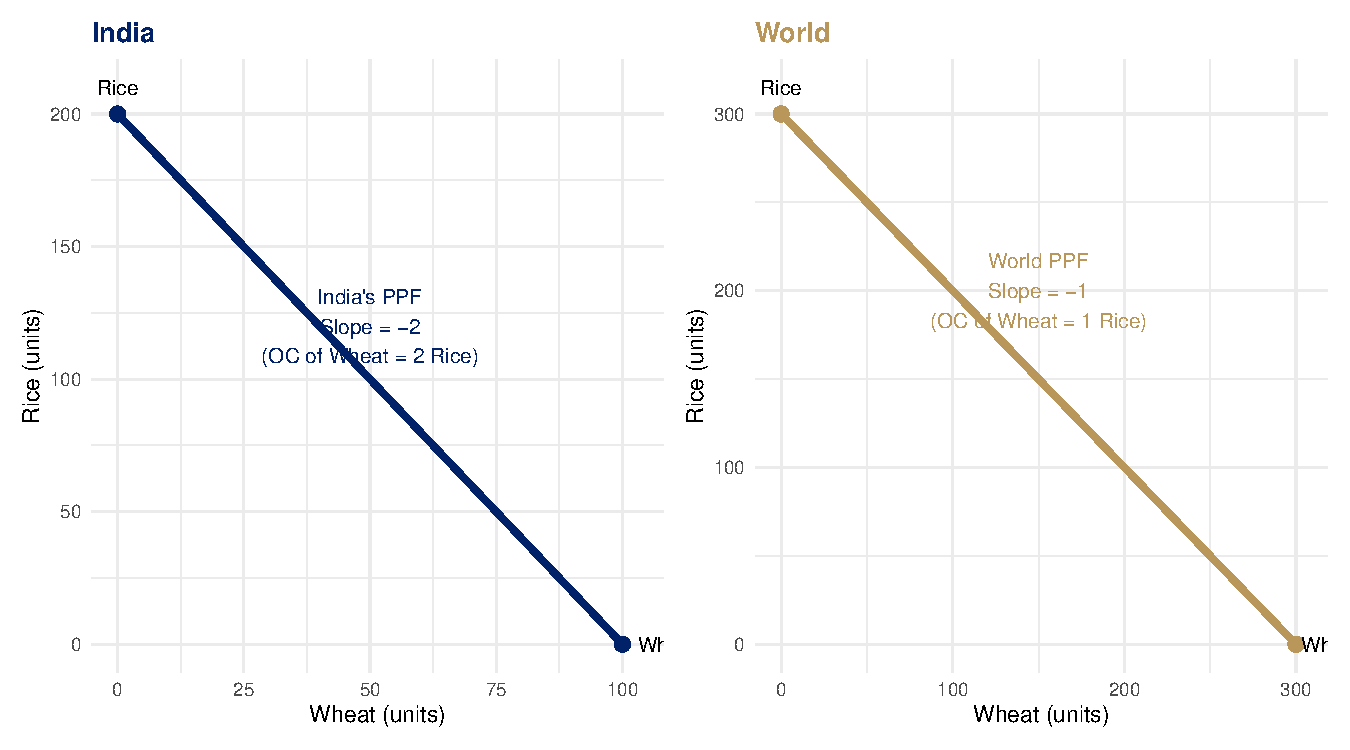
\includegraphics[keepaspectratio]{Lecture04_Comparative_Advantage_files/figure-beamer/fig-ppf-1.pdf}}

}

\caption{\label{fig-ppf}Production Possibility Frontiers: India and
World Source: Author's illustration.}

\end{figure}%
\end{column}
\end{columns}
\end{frame}

\section{Part III: Terms of Trade and Gains from
Trade}\label{part-iii-terms-of-trade-and-gains-from-trade}

\begin{frame}{The Terms of Trade Range}
\phantomsection\label{the-terms-of-trade-range}
For trade to be mutually beneficial, the world price ratio must lie
\textbf{between} the two autarky opportunity costs.

Autarky opportunity costs of Wheat (in terms of Rice):

\[OC_{Wh}^{I} = 2 \text{ Rice} \qquad OC_{Wh}^{W} = 1 \text{ Rice}\]

The \textbf{terms of trade} (price of Wheat relative to Rice) must
satisfy:

\[1 < \frac{P_{Wh}}{P_R} < 2\]

\begin{itemize}
\tightlist
\item
  If \(P_{Wh}/P_R \leq 1\): India would not import Wheat (cheaper to
  produce at home)
\item
  If \(P_{Wh}/P_R \geq 2\): World would not export Wheat (too expensive)
\item
  At any intermediate price, \textbf{both countries benefit}.
\end{itemize}

\textbf{Equilibrium ToT} is determined by relative demand --- say
\(P_{Wh}/P_R = 1.5\).
\end{frame}

\begin{frame}{Gains from Trade: India's Perspective}
\phantomsection\label{gains-from-trade-indias-perspective}
\begin{columns}[T]
\begin{column}{0.4\linewidth}
\textbf{Mechanism:}

\begin{enumerate}
\tightlist
\item
  India \textbf{fully specialises} in Rice → produces (0 Wheat, 200
  Rice)
\item
  Trades Rice for Wheat at world price \(P_{Wh}/P_R = 1.5\)
\item
  \textbf{Consumption} moves to a point \textbf{above} the PPF
\end{enumerate}

The trade possibilities line starts at full specialisation point (0,
200) with slope \(= -1/1.5 \approx -0.67\) (less steep than PPF slope
\(-2\)).

Consumption bundle \textbf{above the PPF} = welfare gain!
\end{column}

\begin{column}{0.6\linewidth}
\begin{figure}

\centering{

\pandocbounded{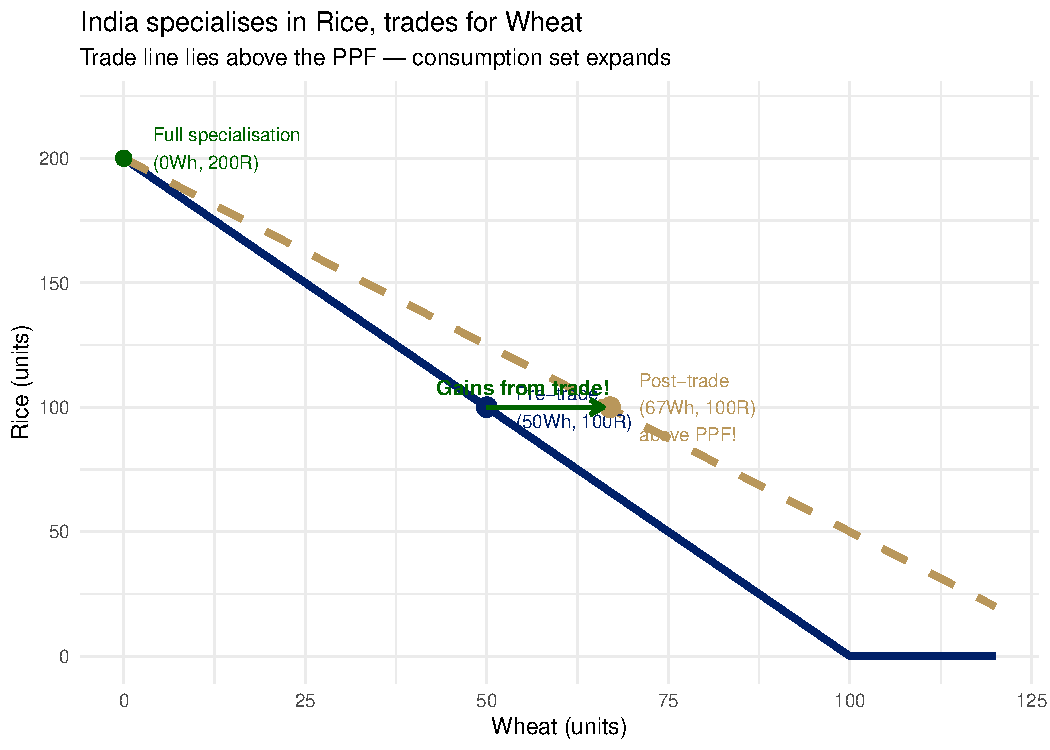
\includegraphics[keepaspectratio]{Lecture04_Comparative_Advantage_files/figure-beamer/fig-gains-1.pdf}}

}

\caption{\label{fig-gains}India: Gains from Trade --- Consuming Beyond
the PPF Source: Author's illustration.}

\end{figure}%
\end{column}
\end{columns}
\end{frame}

\begin{frame}{Quantifying the Gains}
\phantomsection\label{quantifying-the-gains}
\textbf{Before trade} (autarky): India produces and consumes on the PPF
at \((Wh, R) = (50, 100)\)

\textbf{After trade} (at \(P_{Wh}/P_R = 1.5\)): India fully specialises
→ 200 Rice, trades \(107\) Rice for \(\approx 80\) Wheat:
\[(Wh, R) = (80, 93)\]

\textbf{Welfare gain:} more Wheat \emph{and} a larger combined bundle.
The \textbf{real wage} of Indian workers rises.

\textbf{The algebra:} India's income at world prices (fully
specialised):

\[Y^I = P_R \times 200\]

Budget constraint under trade: \(R + 1.5 \cdot Wh = 200\)

Compare with autarky constraint: \(R + 2 \cdot Wh = 200\)

The trade budget line is \textbf{flatter} → larger feasible consumption
set.
\end{frame}

\section{Part IV: Indifference Curves and
Equilibrium}\label{part-iv-indifference-curves-and-equilibrium}

\begin{frame}{Consumer Preferences and Equilibrium}
\phantomsection\label{consumer-preferences-and-equilibrium}
To find the \emph{exact} equilibrium consumption bundle, we need
\textbf{indifference curves (ICs)}.

\begin{columns}[T]
\begin{column}{0.5\linewidth}
\textbf{Properties of ICs:}

\begin{itemize}
\tightlist
\item
  Downward sloping (MRS \textgreater{} 0)
\item
  Convex to origin (diminishing MRS)
\item
  Higher IC = higher utility
\end{itemize}

\textbf{Autarky equilibrium (E1):}

\[\text{MRS} = \frac{P_{Wh}}{P_R} = \frac{a_{LWh}^I}{a_{LR}^I} = 2\]

IC1 is tangent to the PPF at E1.

\textbf{Free-trade equilibrium (E2):}

IC2 is tangent to the \textbf{trade possibilities line} at E2.

Since IC2 is above IC1: \textbf{trade raises welfare}.
\end{column}

\begin{column}{0.5\linewidth}
\begin{figure}

\centering{

\pandocbounded{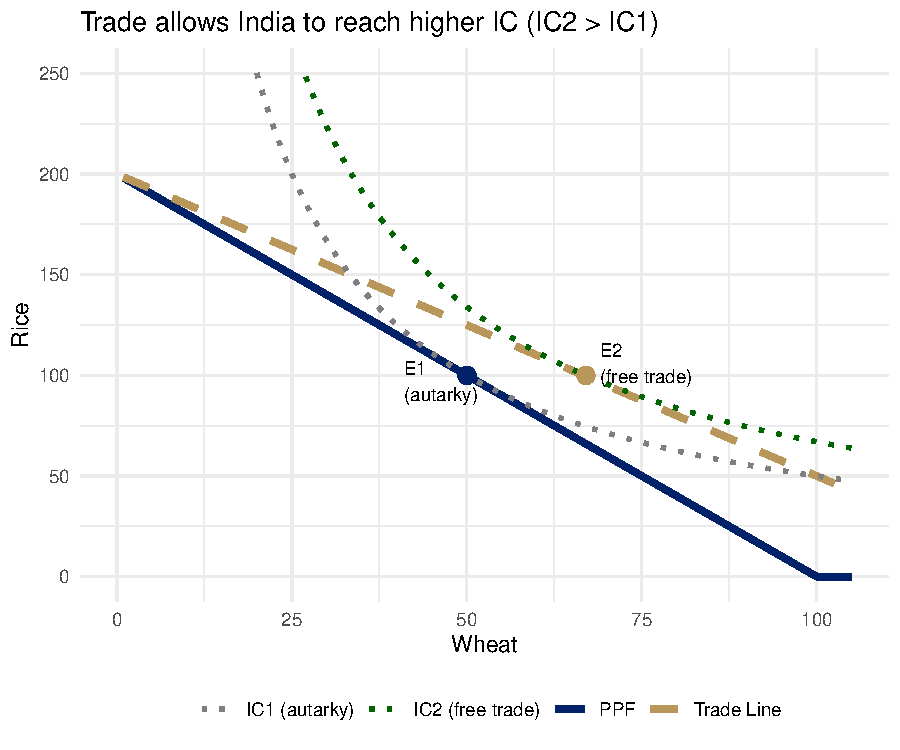
\includegraphics[keepaspectratio]{Lecture04_Comparative_Advantage_files/figure-beamer/fig-ic-ppf-1.pdf}}

}

\caption{\label{fig-ic-ppf}Free Trade Equilibrium: IC tangent to Trade
Possibilities Line Source: Author's illustration.}

\end{figure}%
\end{column}
\end{columns}
\end{frame}

\begin{frame}{Utility Maximisation Under Trade}
\phantomsection\label{utility-maximisation-under-trade}
\textbf{Formal optimisation:}

India maximises \(U(R, Wh)\) subject to the trade budget constraint:

\[\max_{R,\, Wh} \; U(R, Wh) \quad \text{s.t.} \quad P_R \cdot R + P_{Wh} \cdot Wh = P_R \cdot \bar{R}\]

where \(\bar{R} = 200\) (full specialisation output).

\textbf{First-order condition:}

\[\frac{MU_R}{MU_{Wh}} = \frac{P_R}{P_{Wh}} = \frac{1}{1.5}\]

\textbf{Separation of production and consumption decisions:}

Under free trade, India:

\begin{enumerate}
\tightlist
\item
  \textbf{Produces} where \(\text{slope of PPF} = P_R/P_{Wh}\) → full
  specialisation in Rice
\item
  \textbf{Consumes} where \(\text{MRS} = P_R/P_{Wh}\) → tangency of IC
  with trade line
\end{enumerate}

These two points generally differ --- the gap is filled by \textbf{trade
flows}.
\end{frame}

\section{Part V: Assumptions, Extensions, and
Critique}\label{part-v-assumptions-extensions-and-critique}

\begin{frame}{Key Assumptions of the Ricardian Model}
\phantomsection\label{key-assumptions-of-the-ricardian-model}
\begin{longtable}[]{@{}ll@{}}
\toprule\noalign{}
Assumption & Implication \\
\midrule\noalign{}
\endhead
One factor (labour) & Ignores capital, land \\
Constant returns to scale & PPF is linear \\
Perfect factor mobility within country & Instantaneous reallocation \\
Immobile factors across countries & No international migration \\
No transport costs & TOT fully determines trade \\
Perfect competition & No strategic behaviour \\
\bottomrule\noalign{}
\end{longtable}

\note{\textbf{Which matter most?}

\begin{itemize}
\tightlist
\item
  Relaxing \emph{constant returns} → curved PPF, partial specialisation
\item
  Relaxing \emph{one factor} → Heckscher-Ohlin model (Lecture 5)
\item
  Adding \emph{transport costs} → non-traded goods, border effects
\end{itemize}}
\end{frame}

\begin{frame}{The Ricardian Model: What It Gets Right}
\phantomsection\label{the-ricardian-model-what-it-gets-right}
\textbf{Remarkably robust predictions:}

\begin{itemize}
\tightlist
\item
  Countries do specialise along lines of comparative advantage
\item
  Trade raises real incomes on average
\item
  Even the ``least competitive'' country has something to export
\item
  Cannot explain intra-industry trade (→ new trade theory, Lecture 6)
\item
  \textbf{Extensions:} Many goods (Dornbusch-Fischer-Samuelson chain);
  technology changes shift comparative advantage over time
\end{itemize}

\note{\textbf{Empirical support:} Golub \& Hsieh (2000) and Costinot et
al.~(2012) find strong evidence that labour productivity differences
predict export patterns across countries. Predicts complete
specialisation (rarely observed); says nothing about \emph{who} within a
country gains or loses.}
\end{frame}

\section{Part VI: India --- Revealed Comparative
Advantage}\label{part-vi-india-revealed-comparative-advantage}

\begin{frame}{Measuring Comparative Advantage: The Balassa Index}
\phantomsection\label{measuring-comparative-advantage-the-balassa-index}
The \textbf{Revealed Comparative Advantage (RCA)} index (Balassa, 1965):

\[RCA_{ij} = \frac{X_{ij} / X_{i \cdot}}{X_{\cdot j} / X_{\cdot \cdot}}\]

where:

\begin{itemize}
\tightlist
\item
  \(X_{ij}\) = country \(i\)'s exports of good \(j\)
\item
  \(X_{i\cdot}\) = country \(i\)'s total exports
\item
  \(X_{\cdot j}\) = world exports of good \(j\)
\item
  \(X_{\cdot\cdot}\) = world total exports
\end{itemize}

\textbf{Interpretation:}

\begin{itemize}
\tightlist
\item
  \(RCA_{ij} > 1\): country \(i\) has a comparative advantage in good
  \(j\)
\item
  \(RCA_{ij} < 1\): country \(i\) has a comparative disadvantage in good
  \(j\)
\end{itemize}
\end{frame}

\begin{frame}{India's RCA in Agricultural Products}
\phantomsection\label{indias-rca-in-agricultural-products}
\begin{figure}

\centering{

\pandocbounded{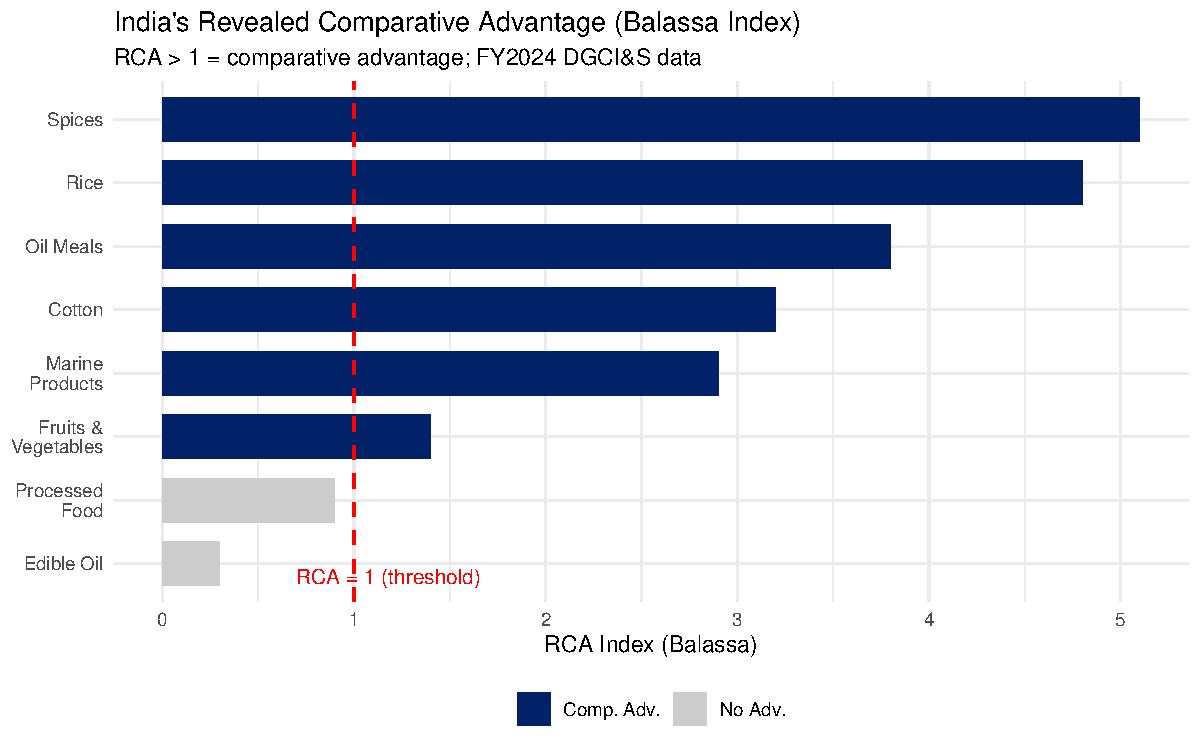
\includegraphics[keepaspectratio]{Lecture04_Comparative_Advantage_files/figure-beamer/fig-rca-1.pdf}}

}

\caption{\label{fig-rca}India: Revealed Comparative Advantage in
Agricultural Products (FY2024) Source: Author's calculations using
DGCI\&S / UN Comtrade data.}

\end{figure}%
\end{frame}

\begin{frame}{India: Rice as the Flagship Export}
\phantomsection\label{india-rice-as-the-flagship-export}
\textbf{India's Rice sector --- Ricardo in practice:}

\begin{itemize}
\tightlist
\item
  India is the \textbf{world's largest rice exporter} (\textgreater22\%
  of global exports, FY2024)
\item
  Rice cultivation is labour-intensive --- India's abundant factor
\item
  \textbf{Relative} labour productivity in rice \textgreater{} relative
  labour productivity in capital-intensive goods
\end{itemize}

\textbf{Policy tension:} September 2023: India imposed a \textbf{25\%
export duty} on non-Basmati white rice → global rice prices spiked 15\%.

\[P_R^{\text{world}} \uparrow \Rightarrow \text{India's ToT deteriorate for future exporters}\]

The ban is welfare-reducing under comparative advantage theory: India
surrenders gains from trade to achieve food security goals.
\textbf{Central tension:} Static efficiency ↔ food security; comparative
advantage ↔ strategic reserves; export competitiveness ↔ domestic price
stability.
\end{frame}

\begin{frame}{Comparative Advantage: Summary}
\phantomsection\label{comparative-advantage-summary}
\textbf{Core results of the Ricardian Model:}

\begin{enumerate}
\tightlist
\item
  Trade is driven by \textbf{relative}, not absolute, productivity
  differences
\item
  Comparative advantage condition:
  \(\frac{a_{LR}^{I}}{a_{LWh}^{I}} < \frac{a_{LR}^{W}}{a_{LWh}^{W}}\)
\item
  Gains from trade: consumption bundle moves \textbf{beyond the PPF}
\item
  Terms of trade must lie between autarky opportunity costs:
  \(OC_R^W < \frac{P_R}{P_{Wh}} < OC_R^I\)
\item
  Both countries gain --- even the absolutely less productive one
\end{enumerate}

\textbf{Empirical verdict:}

\begin{longtable}[]{@{}ll@{}}
\toprule\noalign{}
Prediction & Evidence \\
\midrule\noalign{}
\endhead
Labour productivity → exports & Strong (Costinot et al.~2012) \\
Full specialisation & Weak (partial observed) \\
All workers gain & Mixed (short-run losers exist) \\
India exports rice & Confirmed (RCA = 4.8) \\
\bottomrule\noalign{}
\end{longtable}

\textbf{What Ricardo cannot explain:} \emph{Why} labour productivity
differs (→ H-O model); income distribution effects (→
Stolper-Samuelson); intra-industry trade (→ Lecture 6)
\end{frame}

\section{Appendix}\label{appendix}

\begin{frame}{Additional Resources}
\phantomsection\label{additional-resources}
\textbf{Further Reading}

\begin{itemize}
\tightlist
\item
  \emph{International Economics} --- Salvatore (Ch. 3)
\item
  \emph{International Economics} --- Appleyard \& Field (Ch. 3)
\item
  RBI/DGCI\&S/APEDA databases for latest data
\end{itemize}

\textbf{Key Data Sources}

\begin{itemize}
\tightlist
\item
  DGCI\&S: India's merchandise trade
\item
  RBI: Balance of payments data\\
\item
  APEDA: Agricultural export statistics
\item
  WTO: Tariff and trade databases
\end{itemize}
\end{frame}




\end{document}
